\chapter*{Introduction}

\label{chap:intro}
\addcontentsline{toc}{chapter}{\nameref{chap:intro}}

\fancyhead[LO]{\sffamily\bfseries Introduction} % Print the nearest section name on the left side of odd pages
\fancyhead[RE]{\sffamily\bfseries Introduction} % Print the current chapter name on the right side of even pages




In our quest to describe and understand the world with physics, our intuition tells us to start with the small and the simple before working our way up to larger scales and more complex problems. This is exactly what we do when we are first taught about atomic physics and told to start with the smallest existing atom, the Hydrogen atom. Even before we know about quantum mechanics, we are often taught how to use simple Newtonian mechanics to calculate the circular movement of the Hydrogen electron around the nucleus in the historical Rutherford model. If we now wish to do the same for larger atoms, let us say Carbon for instance, we need to consider the electrostatic forces exerted by the nucleus on each of the 6 electrons as well as between each of the electrons, only to be quickly overcome by a feeling of helplessness at the sight of the equations we would have to solve.


This kind of problems is obviously not restricted to this small example and is actually found in many areas of physics. Would we want to study an ensemble of celestial objects orbiting around a star, electrons in a copper wire, molecules in a gas, atoms in a solid or even how a crowd behaves, a thorough description of these systems would require to account for the motions of all the individual bodies and the interactions between each one of them, leaving us with an absurd amounts of degrees of freedom and equations to solve. This is even more so true as the number of particles can get very large in these problems: a good order of magnitude is the Avogadro number $\mathcal{N}_A = 6.02 \times 10^{23}$, giving the number of carbon 12 atoms in only $12\rm{g}$ of carbon! These problems are regrouped under the denomination ``\textbf{many-body} problems''. 


Actually, many-body problems are not entirely impossible to approach theoretically. To do so, we need to go against our intuition to decompose the system into its elementary components to rather see it as whole to study its \textbf{collective} behavior. This idea is for instance at the core of the field of Thermodynamics which aims to describe ensemble properties of large numbers of particles, such as its temperature, pressure, entropy etc. while not taking any interest in the individual components of the ensemble.

\section*{Quantum many-body physics}

When we study many-body problems where the individual constituents are the (almost) smallest brick of matter, namely electrons and atoms, we enter the realm of \textbf{quantum mechanics}. The key concept to understand when a system requires a quantum treatment is the De Broglie wavelength. In 1923 \cite{debroglie:tel-00006807}, the french physicist Louis de Broglie took the hypothesis of M. Planck and A. Einstein that light could have a corpuscular aspect and turned it around by postulating that matter could behave as a wave with a wavelength $\lambda_{\rm{DB}}$ equal to:

\begin{equation}
    \lambda_{\rm{DB}} = \frac{h}{m\bm{v}}
\end{equation}

\noindent where $m\bm{v}$ is the momentum of the particle that also writes $\hbar \bm{k}$ in quantum mechanics. Strictly speaking, \bm{k} designs a wave vector but we will identify it to the momentum in the rest of this manuscript. Translating this concept to many-body physics, when taking an ensemble of particles at temperature $T$, we can define the average De Broglie wavelength, also known as thermal De Broglie wavelength as:

\begin{equation}
    \lambda_{\rm{DB}} = \frac{h}{\sqrt{2 \pi m \kB T}}
\end{equation}

\noindent If the typical inter-particle density in the many-body ensemble is much larger than the thermal De Broglie wavelength, \ie $\lambda_{\rm{DB}}^3 n \ll 1$, the wave character of the particles plays no role as the different matter waves do not overlap and the system can be properly described using classical physics. On the other hand, when $\lambda_{\rm{DB}}^3 n \sim 1$, the system starts showing quantum behavior. This regime is known as the \textbf{quantum degeneracy} regime. Importantly, this condition is most often met when considering the physics of electrons in condensed matter systems even at room temperature, due to their very small mass and the high densities of particles.

\section*{Interactions in quantum systems}

The key and most essential point of quantum many-body physics is the presence of interactions between the particles. Without interactions, the system is essentially a collection of single particles that we know how to describe and the name ``many-body'' then does not make much sense. Actually, one way of studying the many-body problem is to reduce it to an effective single body problem by using the \textbf{mean-field approximation}. The idea is to approximate the action of every particle of the system on a single one as an averaged single effect, \ie consider the system as a whole and ignore the fact that there are many individual components as suggested before.

While this approach have shown to be very successful, physicist have recently tried to look beyond the mean-field approximation to consider effects between individual particles. As a result, the modern day term ``many-body physics" refers to beyond mean-field approaches that account for the presence of \textbf{correlations} between the individual components of the system. The characterization of these correlations that emerge from the interplay between the inter-particle interactions and the quantum fluctuations is the principal goal of quantum many-body physics and will also be the main point of focus of this thesis. This field of physics indeed remains to this day a largely open field with a lot of unresolved questions concerning systems ranging from solid state physics to neutron stars. We can mention the notable example of low temperature superconductivity studied by Bardeen-Cooper-Schrieffer \cite{bardeen1957theory} (BCS) in 1957 that described the superconducting current as a superfluid of Cooper pairs \cite{cooper1956bound}, where the Cooper pair describes a pair of electrons created by the presence of an interaction effect, in this case the exchange of phonons. The existence of high temperature superconductors remains however unexplained to this day and constitutes a particularly interesting question of many-body physics.

\section*{Cold atoms and quantum simulation}

Even though we have understood that exact analytical approaches are almost always impossible to study quantum many-body systems, we could however think of using numerical techniques and the calculation power of modern-day super computers. Nevertheless, if we wish to consider all kinds of correlations between the particles, the size of the associated Hilbert space grows exponentially with the number of particles considerably limiting the number of particles that can be simulated, roughly a dozen with modern day computers. In a famous paper of 1982 \cite{Feynman1982Simulating}, R. Feynman introduced the concept of \textbf{quantum simulation} by suggesting that quantum phenomena could be simulated using actual quantum components instead of classical computers. The idea is to simulate the system or Hamiltonian of interest with a quantum platform on which we can (1) precisely control all the relevant parameters and (2) easily measure the observable of interest. The technological developments of the past years have made Feynman's idea come to life with increasingly more precise and efficient simulators implemented on a variety of platforms such as ions, superconducting qbits or ultracold gases on which we will focus in this manuscript. 

Contrary to condensed matter systems, ultracold gases are a dilute state of matter in the sense that they typically contain $10^5-10^7$ atoms which is way less than solids, and in larger volumes, resulting in much lower densities. As a result, at room temperature, these gases are far from the quantum degeneracy condition. The idea is then to cool the gas down to very low temperature $\sim \mu \rm{K}$ to increase $\lambda_{\rm{DB}}$ until the system reaches the quantum degenerate regime. When the atoms are indistinguishable  bosons, under a critical temperature, a macroscopic number of atoms occupy the lowest energy state of the system, forming a new state of matter called the \textbf{Bose-Einstein Condensate (BEC)}. Importantly, all the condensed atoms then form a single, \textbf{coherent} matter-wave. 

The field of ultracold atoms was born thanks to the discovery of laser cooling techniques \cite{chu1985three,dalibard1989laser,phillips1982laser} that allowed to reach such low temperatures and led to the observations of the first BECs by the teams of E. Cornell \cite{anderson1995observation} and W. Ketterle \cite{davis1995bose} in 1995. From this day, ultracold atoms and Bose-Einstein Condensates have been the subject of many experiments and brought a large variety of important results and several Nobel prizes.

Ultracold atoms are actually perfectly suited to study condensed matter as it is relatively easy to create all sorts of potentials to trap the atoms using laser light, with the notable example of optical lattices \cite{bloch2005ultracold} that reproduces the crystalline structure of condensed matter. Another interesting properties of ultracold atoms is that the strength of the interactions can be tuned using Feshbach resonance \cite{chin2010feshbach,feshbach1958unified}. We thus have a system in which we can control the number of particles, the properties of the crystal-like potential such as its geometry and the distance between the sites and finally the strength of interactions, thus perfectly fulfilling the first condition for it to be a good quantum simulator of famous condensed matter models such as the Fermi- and Bose-Hubbard models for fermions and bosons respectively, or the Ising model. 

\section*{Time-Of-Flight measurements and the momentum distribution}

This level of control on the parameters of the simulated Hamiltonian would of course be useless if it were impossible to measure the properties of the system. One other significant asset of ultracold atoms in optical lattices systems is that they are actually easy to probe. Recent experiments typically fall into two categories, depending on what quantity the aim at measuring:

\begin{itemize}
 \item The position of the atoms, \ie the distribution of the atoms into the different lattice sites. This is done using quantum gases microscopes \cite{bakr2009quantum}, capable of detecting the fluorescence of individual atoms trapped in the lattice.
 \item The momentum of the atoms. This can be done using Bragg spectroscopy \cite{stenger1999} that we will not detail here, or Time-Of-Flight (TOF) techniques. The experiment that we will describe in this manuscript belongs to this last category.
\end{itemize}

The concept of Time-Of-Flight measurements is actually quite simple. The idea is to abruptly turn off the trapping potential to let the atoms fall under the effect of gravity and measure their positions $\bm{r}$ after a given TOF $t_{\rm{TOF}}$. In a very simple picture with classical particles that do not interact during the TOF, this position gives information about the in-trap momentum of the particle through the simple \textbf{ballistic relation}:

\begin{equation}
    \hbar \bm{k} = \frac{m \bm{r}}{t_{\rm{TOF}}}
\end{equation}

\noindent The situation is in reality more complex when accounting for the wave nature of the particles. This will be discussed in great details throughout this manuscript, but we can keep for now this simple image.

There are in fact many motivations to measure the momentum distribution to study ultracold gases and many-body physics as a whole. To begin, the momentum distribution was historically used to detect the presence of Bose-Einstein Condensation as illustrated on Fig.-\ref{fig:1st_BEC}. The BEC manifest itself by the presence of sharp peak around zero momentum with a small width set by Heisenberg uncertainty principle as the atoms are spatially localized. The momentum distribution can also be used to determine the \textbf{coherence} properties of the system, that are themselves greatly influenced by the interactions and the induced correlations between the particles. This can be understood with an analogy with optics in which far-field interference experiments are used to characterize the spatial and temporal coherence properties of a light source. With ultracold atoms, the light waves are replaced by matter-waves and the far-field regime of observation analog to the momentum distribution of the gas. The momentum distribution is also perfectly suited to study excitations signaled in momentum space by the dispersion relation from which a variety of information can be obtained \NOTE{refs}.


\begin{figure}
    \centering
    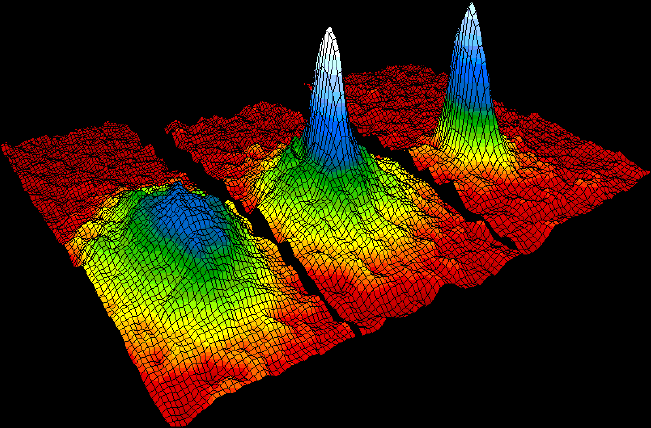
\includegraphics[width=0.7\textwidth]{Fig/Intro/BEC.png}
    \caption[Momentum distribution across Bose-Einstein Condensation]{Bose-Einstein Condensation. As temperature diminishes, the momentum distribution gets increasingly peaked around zero momentum.}
    \label{fig:1st_BEC}
\end{figure}


Last but not least, the momentum distribution also contains signatures of more complex interaction-induced correlation patterns between several individual particles. One of the most simple and famous example of such correlations are opposite momentum pairing effects. This is notably the case for the two electrons in Cooper pair as discussed earlier, as well as for the \textbf{quantum depletion} of a BEC. The quantum depletion designates the fraction of atom removed from the condensate by the effect of interactions and quantum fluctuations and is then a classic and conceptually simple example of a many-body effect. While the quantum depletion has already been observed before \cite{chang2016,lopes2017,xu2006}, there have been no direct observation of the opposite momentum pairing of quantum depleted atoms. Obtaining this result will be the main point of focus of this manuscript.

\section*{Metastable Helium and electronic detection}

Ideally, we would like to characterize all kinds of correlations present in the system, \ie correlations involving an arbitrary amount of particles. This is only achievable if a method is available to measure the momentum of each of the individual atoms of the gas. This is usually not the case in most ultracold experiments where the optical imaging techniques only allow to measure the \textbf{momentum density} of the gas rather than the full \textbf{momentum distribution}. In the early 2000s, the team lead by D. Boiron, C. Westbrook and A. Aspect at Institut d'Optique pioneered a new electronic detection technique exploiting the properties of the metastable state of the Helium atom that they managed to bring to quantum degeneracy in 2001 \cite{robert2001bose}. This detection technique has the amazing advantage of having a \textbf{single-atom} sensitivity, making it perfectly suited for the measurement of correlations in momentum space.

A second metastable Helium experiment was then built at Institut d'Optique under the direction of David Clément starting in 2011, with the observation Bose-Einstein condensation in 2015 \cite{bouton2015fast}. This new experiment implemented a new cooling sequence allowing to produce a BEC in $\sim 6\rm{s}$ instead of $\sim 30\rm{s}$ on the historical experiment, thus significantly speeding up the data acquisition time for momentum correlation measurements.

\section*{Optical lattices and the superfluid-to-Mott insulator transition}

The other specificity of this experiment is the use of optical lattices, from which the name of the team ``Helium Lattice'' derives. Optical lattices are particularly suited to study many-body, strongly interacting systems as the lattice potential locally increases the density and in turn the interactions, making phenomenon like quantum depletion even more pronounced than in regular harmonic traps. In addition, the Bose-Hubbard model predicts the existence of a phase transition from a superfluid phase to an insulating phase when the depth of the lattice potential increases known as the superfluid-to Mott insulator transition, first observed with cold atoms by I. Bloch team in 2002 \cite{greiner2002quantum}. Studying momentum correlations all across the superfluid-to Mott insulator transition sets the general frame of the work presented in this manuscript conducted during my time as an intern and then PhD student in the Helium Lattice team that I the chance to join in 2018.

\section*{Outline of the manuscript}

This manuscript is organized in five chapters. All chapters but the final one are centered around the common topic of the \kmk correlations in the quantum depletion of weakly-interacting lattice Bose gas.

\begin{itemize}
    \item The first chapter is dedicated to presenting the proper formalism to study quantum correlations. The concept of correlation functions is first introduced in the context of Optics and then extended to atomic physics. We then present the main lines of the Bogoliubov theory of the homogeneous weakly-interacting Bose gas and show what the quantum depletion is and where does the \kmk pairing comes from. Finally, we discuss some recent numerical calculations \cite{butera2020} of the correlations in the Bogoliubov theory for trapped systems, before presenting the essential experimental ingredients to observe the \kmk pairs.
    \item The second chapter is also a theoretical one and discusses the Bose-Hubbard model of bosons trapped in a 3D optical lattice. We explain what the superfluid-to-Mott insulator transition is and discuss the conditions under which the in-trap momentum distribution of the gas can be properly measured using a TOF technique, as well a the observability of the \kmk pairs of the quantum depletion in this system.
    \item The third chapter describes our experimental apparatus, namely the sequence used to produce a BEC of metastable Helium and the detection technique. In a second time, we present two experimental measurements aimed at proving the points raised in Chapter \ref{sec:chapter_2}, one proving that we are able to adiabatically prepare an arbitrary state of the Bose-Hubbard model and a second one measuring beyond-mean field two-body collision effects happening during the TOF to prove that they are negligible in usual experimental conditions and therefore not detrimental to our measurement of the momentum distribution. 
    \item The fourth chapter details our experimental observation of the \kmk pairs of the quantum depletion. We describe the numerical procedure to analyze the data and study the characteristics of the experimental correlation signals in light of Bogoliubov theory: width, amplitude and dependency to temperature. We then perform complementary analysis of the data to obtain results leading towards showing the presence of entanglement in our system: we observe a relative number squeezing measurement between modes $\bm{k}$ and $-\bm{k}$, as well as a violation of the Cauchy-Schwarz inequality. Finally, we discuss some preliminary results on the evolution of the correlation signals with momentum $k$.
    \item The fifth and last chapter is separate from the rest of this manuscript and concerns a different project that was lead during this thesis, the measurement of Tan's contact in 1D gases. We first present what Tan's contact is and present some main results of a recent theoretical study \cite{yao2018tan} of the evolution of contact with temperature and interaction strength for trapped 1D bosons, before showing how our experimental apparatus can be adapted for this kind of measurements. We then present the procedure used to extract the contact from the raw experimental data and discuss the first preliminary results and their discrepancy with theory. We conclude by giving a few possible explanations for these discrepancies and discussing what we plan on doing next.
\end{itemize}









